\documentclass[aspectratio=169,11pt]{beamer}
\usepackage{teaching_slides}

\title[L13a - Censoring and Tobit]{ Econometrics I}
\subtitle{Lecture 13a: Censored Outcomes and the Tobit Model}
\author{Chris Conlon \\NYU Stern}
\date{Fall 2026}

% New deck (Fall 2026). Readings: Hansen Ch. 27; Wooldridge Ch. 17.
% Figures/tables simulated with known ground truth: ldv_sims.R (Part A).
% Workbook: inclass_session13.Rmd

\begin{document}
\maketitle

\begin{frame}{Session 13: outcomes that are not ``a number on the real line''}
\begin{itemize}
	\item Weeks 2--11 modeled $\E[y \mid x]$ for a continuous $y$. Week 12 handled $y \in \{0, 1\}$ and
	the case where $y$ is only \emph{observed} for a selected subsample (Heckman).
	\medskip
	\item Today, three more shapes of $y$ that business data take, each with its own likelihood:
	\begin{enumerate}
		\item \alert{Censored}: spending is zero for half the sample, or income is top-coded at \$250k. (This deck.)
		\item \alert{Durations}: months until a customer churns, days until a loan defaults, and the clock
		is still running for many of them when the data end. (Deck b.)
		\item \alert{Counts}: purchases, visits, patents, complaints. Non-negative integers with lots of zeros. (Deck c.)
	\end{enumerate}
	\medskip
	\item Common thread: OLS on $y$ answers a question, but usually not the one you asked. Writing down
	the likelihood forces you to say what $y$ is, and then Week 12's MLE machinery does the rest.
	\medskip
	\item Readings: Hansen Ch.~27; Wooldridge Ch.~17 (censoring), 22 (durations), 19 (counts).
\end{itemize}
\end{frame}


\begin{frame}{Censoring versus truncation}
\begin{center}
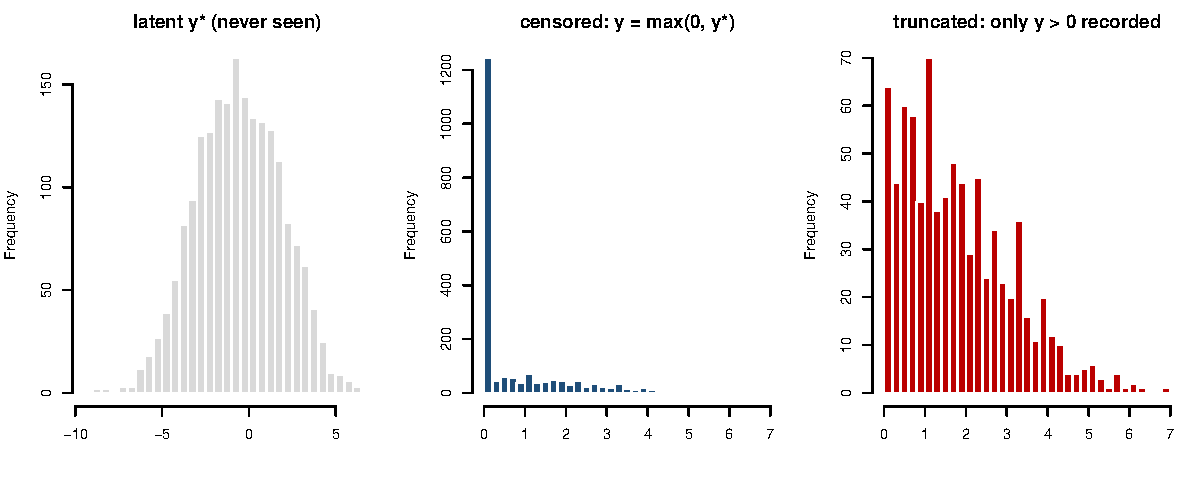
\includegraphics[width=.7\textwidth]{fig_tobit_trunc.pdf}
\end{center}
\vspace{-.2cm}
\begin{itemize}
	\item \alert{Censored}: every unit is in the data, but $y$ is recorded at a limit when $y^*$ is past it.
	You \emph{see} the pile-up: spending ($0$), top-coded income, demand at a stockout.
	\item \alert{Truncated}: units past the limit are \emph{not in the data at all}: only customers who
	bought appear in the transactions file. Week 12's selection problem with the rule known.
	\item Censoring is milder: the zeros carry information.
\end{itemize}
\end{frame}


\begin{frame}{The model}
\begin{align*}
	y_i^* = x_i'\beta + \varepsilon_i, \qquad \varepsilon_i \mid x_i \sim N(0, \sigma^2), \qquad
	y_i = \max(0, y_i^*).
\end{align*}
\begin{itemize}
	\item $y^*$ is the \alert{latent} variable: desired spending, which can be negative (``I would pay
	to not have this''). We observe it only when it is positive.
	\medskip
	\item Two readings of the same equation:
	\begin{itemize}
		\item \alert{Genuine censoring}: $y^*$ is real and interesting (true income behind a top-code).
		The estimand is $\beta$.
		\item \alert{Corner solution}: $y^*$ is a device; the economic object is the observed $y$
		(spending is zero because the optimum is a corner). The estimand is $\partial\E[y \mid x]/\partial x$.
	\end{itemize}
	Same likelihood, different marginal effect. Decide which you are before reporting a number.
	\medskip
	\item Tobin (1958) wrote this down for household durable spending; hence ``Tobit.''
\end{itemize}
\end{frame}


\begin{frame}{Running example: spending on a product category}
\begin{itemize}
	\item $2{,}000$ households. $x$ is standardized income. Latent spending
	$y^* = -0.5 + \alert{1.5}\,x + \varepsilon$, $\varepsilon \sim N(0, 2^2)$, observed $y = \max(0, y^*)$.
	\medskip
	\item About $59\%$ of households spend nothing. That is not unusual: most product categories are
	bought by a minority of households in any given period.
	\medskip
	\item Ground truth: $\beta = 1.5$, $\sigma = 2$. We will run the regressions people actually run,
	and then the right one.
\end{itemize}
\end{frame}


\begin{frame}{What OLS does}
\begin{center}
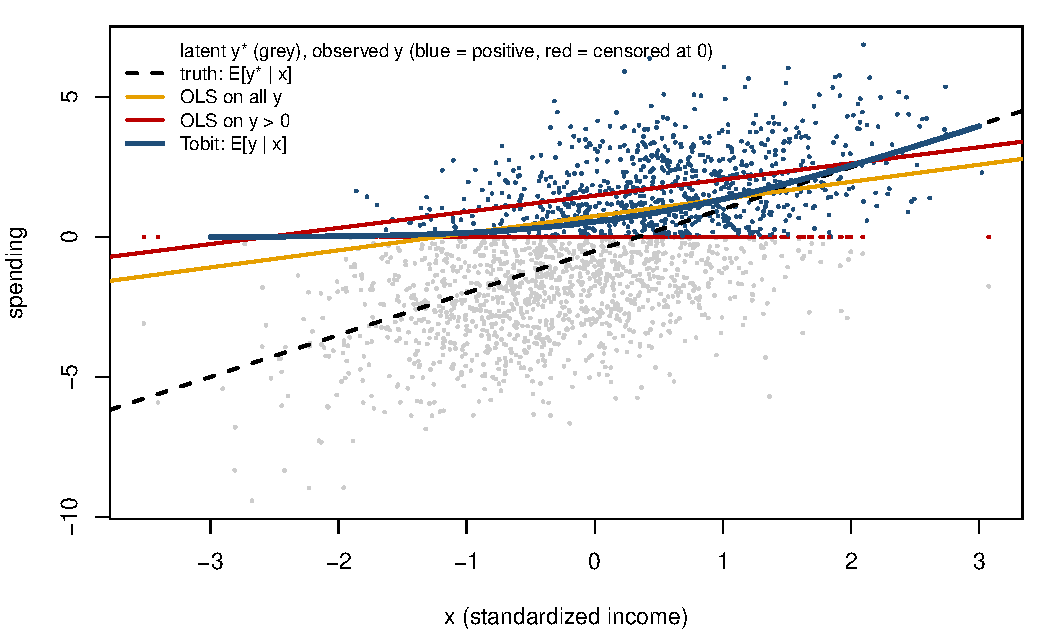
\includegraphics[width=.62\textwidth]{fig_tobit_scatter.pdf}
\end{center}
\vspace{-.3cm}
{\small Grey: the latent $y^*$ nobody sees. Red: households censored at zero. OLS on everyone is pulled flat by the
zeros; OLS on buyers only is pulled flat by truncation from below. Both are less than half the truth.}
\end{frame}


\begin{frame}{Why both OLS regressions fail}
\begin{itemize}
	\item \alert{OLS on all $y$.} We are fitting $\E[y \mid x]$, and
	\begin{align*}
		\E[y \mid x] = \Pr(y^* > 0 \mid x)\cdot \E[y^* \mid x, y^* > 0] = \Phi\!\left(\tfrac{x'\beta}{\sigma}\right) x'\beta + \sigma\,\phi\!\left(\tfrac{x'\beta}{\sigma}\right),
	\end{align*}
	which is \emph{nonlinear} in $x$ and flatter than $x'\beta$ wherever censoring bites. A line through it
	has slope $\approx \beta \cdot \Pr(y > 0)$. Here that is $1.5 \times 0.41 \approx 0.6$.
	\medskip
	\item \alert{OLS on $y > 0$.} Conditioning on $y^* > 0$ means conditioning on $\varepsilon > -x'\beta$.
	Low-$x$ households are in the sample only if they drew a large positive $\varepsilon$:
	\begin{align*}
		\E[y \mid x, y > 0] = x'\beta + \sigma\,\lambda\!\left(\tfrac{x'\beta}{\sigma}\right), \qquad \lambda(z) = \frac{\phi(z)}{\Phi(z)} .
	\end{align*}
	The omitted term is decreasing in $x$: the same inverse Mills ratio as Heckman, with the selection
	equation known exactly.
	\medskip
	\item Neither is ``biased a little.'' Both are wrong by a factor that depends on how much censoring there is.
\end{itemize}
\end{frame}


\begin{frame}{The Tobit likelihood: a probit and a regression glued together}
Each observation contributes one of two pieces:
\begin{align*}
	\ell(\beta, \sigma) = \sum_{i:\, y_i = 0} \ln \underbrace{\Big[1 - \Phi\!\Big(\tfrac{x_i'\beta}{\sigma}\Big)\Big]}_{\Pr(y^*_i \le 0)}
	\ +\ \sum_{i:\, y_i > 0} \ln \underbrace{\Big[\tfrac{1}{\sigma}\,\phi\!\Big(\tfrac{y_i - x_i'\beta}{\sigma}\Big)\Big]}_{\text{normal density at } y_i}
\end{align*}
\begin{itemize}
	\item Censored observations enter through a \alert{probability} (we know only that $y^* \le 0$);
	uncensored ones through a \alert{density} (we know $y^*$ exactly). Mixing the two is what makes it
	a censored model rather than a probit or a regression.
	\medskip
	\item Truncated regression drops the first sum and divides the density by $\Phi(x_i'\beta/\sigma)$:
	less information.
	\item Concave in $(\beta/\sigma, 1/\sigma)$ (Olsen 1978), so Newton converges from anywhere. Only
	$\beta/\sigma$ enters the probit part, so a probit on $\mathbb{1}\{y > 0\}$ estimates $\beta/\sigma$: a useful check.
\end{itemize}
\end{frame}


\begin{frame}{Estimates on the simulated households}
\begin{center}
\small
\begin{tabular}{lccccc}\toprule
 & OLS on $y$ (all) & OLS on $y$ ($y > 0$ only) & Tobit MLE & Probit on $\mathbb{1}\{y>0\}$ & OLS on $y^*$ (infeasible) \\ \midrule
Slope on $x$ (truth $= 1.5$) & 0.612 & 0.577 & 1.487 & 0.778 $= \beta/\sigma$ & 1.456 \\
 & (0.024) & (0.050) & (0.062) & (0.037) & (0.045) \\
Intercept (truth $= -0.5$) & 0.748 & 1.477 & -0.516 & -0.281 & -0.567 \\
$\hat\sigma$ (truth $= 2$) & 1.064 & 1.224 & 1.941 & --- & 2.011 \\
$N$ & 2000 & 819 & 2000 & 2000 & 2000 \\
\bottomrule\end{tabular}

\end{center}
\medskip
\begin{itemize}
	\item Tobit recovers $\beta$ and $\sigma$. The probit on the zero/positive split recovers $\beta/\sigma = 0.75$.
	\item The last column is what you would get if you could see $y^*$: the goal, and Tobit gets there.
\end{itemize}
\end{frame}


\begin{frame}{Three marginal effects, and which one you want}
\begin{columns}[T]
\begin{column}{0.5\textwidth}
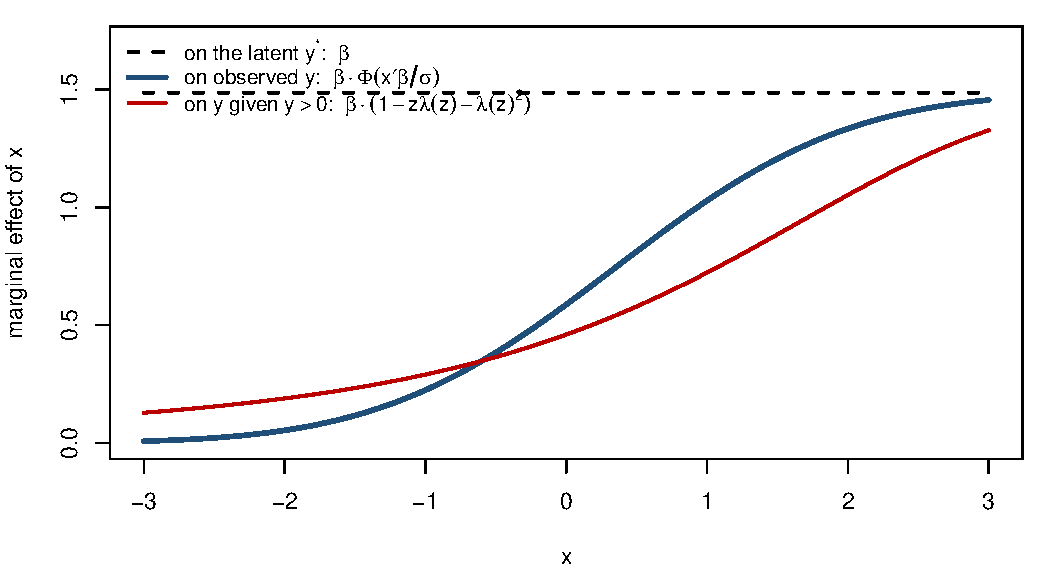
\includegraphics[width=\textwidth]{fig_tobit_me.pdf}
\end{column}
\begin{column}{0.5\textwidth}
\small
\begin{itemize}
	\item \alert{On $y^*$}: $\beta$. Report this if the latent variable is the object (top-coded income).
	\item \alert{On observed $y$}: $\beta \cdot \Phi(x'\beta/\sigma)$, the effect on expected spending
	including households moved off zero. Report this for corner solutions. It is $\beta$ times the
	share of buyers, so it varies with $x$.
	\item \alert{On $y$ given $y > 0$}: $\beta\,[1 - z\lambda(z) - \lambda(z)^2]$, $z = x'\beta/\sigma$.
	The intensive margin among current buyers.
	\item McDonald--Moffitt (1980): the second is the third (intensive) plus the extensive margin.
\end{itemize}
\end{column}
\end{columns}
\end{frame}


\begin{frame}{Assumptions that do the work}
\begin{itemize}
	\item \alert{Normality} and \alert{homoskedasticity} of $\varepsilon$. Unlike OLS, these are not just
	for standard errors: the Tobit MLE is \emph{inconsistent} if either fails, because the probability
	$\Pr(y^* \le 0 \mid x)$ is computed from the assumed distribution.
	\medskip
	\item Practical check: does the probit on $\mathbb{1}\{y > 0\}$ give roughly $\hat\beta_{Tobit}/\hat\sigma$?
	If not, the two pieces of the likelihood disagree about the model.
	\medskip
	\item \alert{The zeros are the same process as the positives.} Tobit says a household spends zero
	because its latent demand is low. If zeros come from a \emph{different} decision (never shops
	this category; the store was out of stock), you want a two-part or hurdle model: a probit for
	``any?'' and a regression for ``how much, given any?'' with separate coefficients. The count-data
	deck does the same thing for integers.
	\medskip
	\item Heteroskedasticity and non-normality can be handled (CLAD, Powell 1984, needs only a median
	restriction), at the cost of efficiency and software convenience.
\end{itemize}
\end{frame}


\begin{frame}{Variations you will meet}
\begin{itemize}
	\item \alert{Top-coding / right-censoring.} $y = \min(y^*, c)$. Same likelihood with $\Phi$ replaced
	by $1 - \Phi$ in the censored piece. Wages in public-use files, damage awards, capped insurance claims.
	\medskip
	\item \alert{Two-sided censoring.} Scores bounded at $0$ and $100$; shares in $[0, 1]$.
	\medskip
	\item \alert{Censoring points that vary by $i$.} Each unit has its own limit $c_i$ (a customer's
	credit limit; a plant's capacity). Fine, as long as $c_i$ is known and exogenous.
	\medskip
	\item \alert{Interval censoring.} You know $y^* \in (a_i, b_i]$: income reported in brackets.
	The likelihood piece is $\Phi(b) - \Phi(a)$. This is also how duration data with grouped time work.
	\medskip
	\item \alert{Censoring in time} is the whole subject of the next deck.
\end{itemize}
\end{frame}


\begin{frame}[fragile]{In practice}
Tobit is a left-censored normal regression, which is what \texttt{survreg} in the \texttt{survival} package
(shipped with R) estimates:
\begin{lstlisting}
library(survival)
tob <- survreg(Surv(y, y > 0, type = "left") ~ x, data = d, dist = "gaussian")
coef(tob); tob$scale                      # beta and sigma
feglm(I(y > 0) ~ x, d, family = binomial("probit"))   # check: should be about beta / sigma
\end{lstlisting}
\begin{lstlisting}[language=Python]
# statsmodels has no Tobit; the likelihood is eight lines with scipy.optimize
from scipy.stats import norm
def nll(th, y, X):
    b, s = th[:-1], np.exp(th[-1]); xb = X @ b
    return -(np.where(y > 0, norm.logpdf(y, xb, s), norm.logcdf(-xb / s))).sum()
\end{lstlisting}
\begin{itemize}
	\item Marginal effects on observed $y$: multiply $\hat\beta$ by the average of $\Phi(x_i'\hat\beta/\hat\sigma)$.
\end{itemize}
\end{frame}


\begin{frame}{Recap}
\begin{itemize}
	\item Censored: you see the pile-up at the limit. Truncated: the units past the limit are gone.
	\medskip
	\item OLS on censored $y$ estimates a flattened slope; OLS on the positives has a Heckman-style
	omitted term. Neither is close.
	\medskip
	\item Tobit is a probit for the censored observations glued to a normal regression for the rest.
	It needs normality and homoskedasticity for \emph{consistency}, not just for inference.
	\medskip
	\item Three marginal effects. Say whether your question is about the latent variable or the
	observed one before you pick.
	\medskip
	\item If the zeros are a different decision, use a two-part model. The count deck picks that up.
\end{itemize}
\end{frame}

\end{document}
